In this section we explain the technological parameters estimation and analysis for a single MOSFET and NAND-2 input.
\subsection{Technological Parameters}
We have estimated necessary technological parameters in order to evaluate:
\begin{itemize}
\item Static power
\item Dynamic power
\item Input-to-output delay
\item Maximum frequency
\end{itemize}
The static power can be evaluated as shown below
\begin{equation}
P_{static}=V_{DD} \cdotp I_{leak}
\end{equation}
where $I_{leak}$ is the leakage current and $V_{DD}$ is the voltage supply. \\The dynamic power can be computed as
\begin{equation}
P_{dynamic}= \alpha \cdotp C_{gate} \cdotp V_{DD}^2 \cdotp f
\end{equation}
where $\alpha$ is the switching activity, $\alpha \cdotp C_{gate}$ is the switching capacitance and $f$ is the frequency. \\The oxide capacitance per unit length is the same for pMOS and nMOS transistors.
\begin{equation}
C_{OX}=\frac{10^9 \cdotp (\epsilon_0 \cdotp \epsilon_r)}{t_{OX}} \cdotp L_{eff} \quad [pF/\mu m]
\end{equation}
where $L_{eff}$ is the effective gate length and $t_{OX}$ is the thickness of the oxide. \\The input capacitance of nMOS and pMOS transistors per unit length are:
\begin{eqnarray}
C_{in_N}=C_{OX}+C_{overlapN} \quad [pF/\mu m]\\
C_{in_P}=C_{OX}+C_{overlapP} \quad [pF/\mu m]
\end{eqnarray}
where the two overlap capacitances are due to the overlap size between the gate and drain/source areas:
\begin{eqnarray}
C_{overlapN}=10^6 \cdotp C_{GDOn} \quad [pF/\mu m]\\
C_{overlapP}=10^6 \cdotp C_{GDOp} \quad [pF/\mu m]
\end{eqnarray}
The junction capacitances between source and drain are:
\begin{eqnarray}
C_{jN}=C_{bottomN} + C_{sidewallN} \quad [pF/\mu m]\\
C_{jP}=C_{bottomP} C_{sidewallP} \quad [pF/\mu m]
\end{eqnarray}
$C_{bottom}$ is the capacitance due to the area of the pool of the source/drain and $C_{sidewall}$ is the one due to the edge of the same pool.
\begin{eqnarray}
C_{bottomN}=C_{j0_N} \cdotp \Bigl(1+ \frac{V_{DD}}{2 \cdotp P_{bN}} \Bigr)^{-M_{jN}} \cdotp 2.5 \cdotp L_{drawn} \quad [pF/\mu m]\\
C_{bottomP}=C_{j0_P} \cdotp \Bigl(1+ \frac{V_{DD}}{2 \cdotp P_{bP}} \Bigr)^{-M_{jP}} \cdotp 2.5 \cdotp L_{drawn} \quad [pF/\mu m]\\
C_{sidewallN}=10^6 \cdotp C_{sw_N} \cdotp \Bigl(1+ \frac{V_{DD}}{2 \cdotp P_{bswN}} \Bigr)^{-M_{jswN}} \quad [pF/\mu m]\\
C_{sidewallP}=10^6 \cdotp C_{sw_P} \cdotp \Bigl(1+ \frac{V_{DD}}{2 \cdotp P_{bswP}} \Bigr)^{-M_{jswP}} \quad [pF/\mu m]
\end{eqnarray}
Moreover for the estimation of parasitic capacitances $C_{jN}$ and $C_{jP}$, it is necessary to evaluate the perimeter.
\begin{eqnarray}
\text{perim}_N=2 \cdotp \text{lungh\_diff} + W_N [\mu m]\\
\text{perim}_P=2 \cdotp \text{lungh\_diff} + W_P [\mu m]
\end{eqnarray}
We consider only one side for the $W$, because the internal one doesn't touch a conductor, but just a spatial charge. \\Therefore $C_{jN}$ and $C_{jP}$ are:
\begin{eqnarray}
C_{jN}=C_{bottomN} \cdotp W_N + C_{sidewallN} \cdotp \text{perim}_N \quad [pF]\\
C_{jP}=C_{bottomP} \cdotp W_P + C_{sidewallP} \cdotp \text{perim}_P \quad [pF]
\end{eqnarray}
For the leakage current we consider two factors
\begin{itemize}
\item \textbf{Subthreshold current}: is the leakage current that flows drain/source when $V_{gate_{nMOS}}=0$ and $V_{gate_{pMOS}}=V_{DD}$ as shown in figure \ref{fig:ds_leakage}.
\begin{figure}[htbp]
\begin{center}
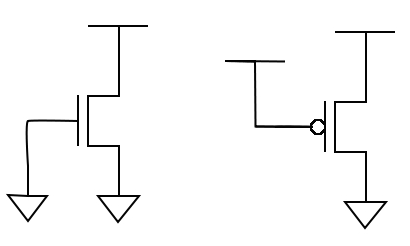
\includegraphics[width=0.5\textwidth]{img/mos_off.png}
\caption{Leakage drain/source current when MOS are off}
\label{fig:ds_leakage}
\end{center}
\end{figure}

\item \textbf{Gate Current}: is the leakage current that flows from drain and source to gate or viceversa when drain and source are tied at the same potential and gate is tied at the opposite potential for nMOS and pMOS as shown in figure \ref{fig:gate_leakage}.
\begin{figure}[htbp]
\begin{center}
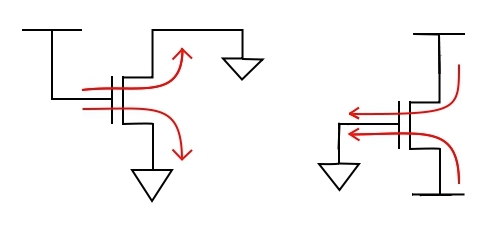
\includegraphics[width=0.5\textwidth]{img/mos_gate.jpg}
\caption{Leakage gate current}
\label{fig:gate_leakage}
\end{center}
\end{figure}

\end{itemize}

\subsection{Dynamic Analysis}
For the 2-input NAND in CMOS technology, the architecture is shown in figure \ref{fig:nand-2}.
\begin{figure}[htbp]
\begin{center}
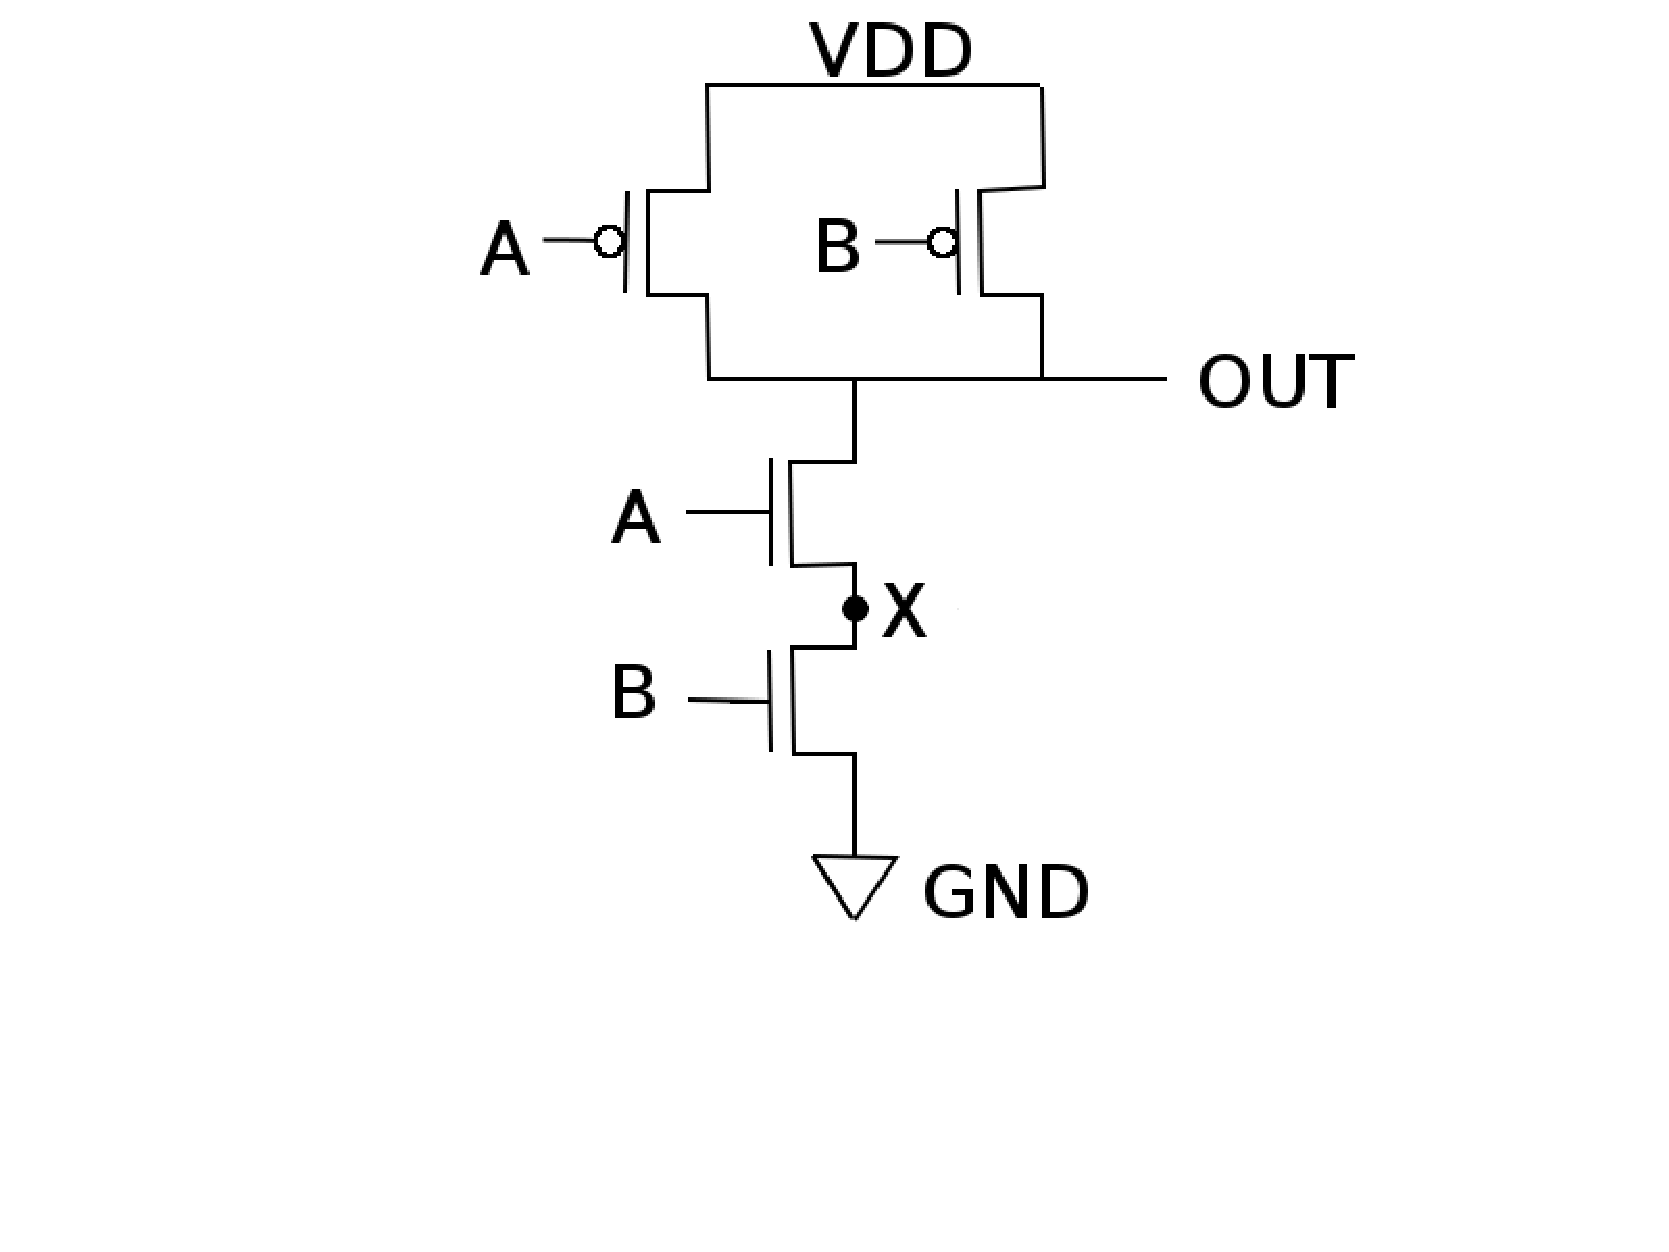
\includegraphics[width=0.5\textwidth]{img/Nand.pdf}
\caption{CMOS 2-input NAND architecture}
\label{fig:nand-2}
\end{center}
\end{figure}
In order to compute the dynamic power, we have to calculate the total switching capacitance. \\We have to consider three different capacitance:
\begin{itemize}
\item $C_{IN}$ is the input capacitance associate at only one input
\begin{equation}
C_{IN}= C_{OX} \cdotp 2W_N \cdotp L_{eff} + C_{OX} \cdotp W_P \cdotp L_{eff} + 2C_{overlapN}+ 2C_{overlapP} \quad [pF]
\end{equation}
\item $C_{OUT}$ is the output capacitance
\begin{equation}
C_{OUT}=C_{jN} + 2C_{jP} \quad [pF]
\end{equation}
$C_{jP}$ is multiplied by 2 because we have different pools for the two drains.
\item $C_{INT}$ is the internal capacitance between the two nMOS transistors in the pull-down network
\begin{equation}
C_{INT}=C_{jN} \quad [pF]
\end{equation}
We have only one $C_{jN}$ because we consider that source and drain are common for the two nMOS.
\end{itemize}
To calculate the dynamic power is necessary to compute the switching activity for each node, using the probability that each node is equal to one.
\begin{equation}
P_{X1}=\frac{P_A \cdotp (1-P_B)}{1-(1-P_A) \cdotp (1-P_B)}
\end{equation}
$P_{X1}$ is the probability that the internal node in equal to one. The probability $P_{OUT}$ at the output node is
\begin{equation}
P_{OUT}=1-(1-P_A) \cdotp (1-P_B)
\end{equation}
The switching activities are computed from probabilities as follow
\begin{eqnarray}
\alpha_A = P_A \cdotp (1-P_A)\\
\alpha_B = P_B \cdotp (1-P_B)\\
\alpha_X1 = P_{X1} \cdotp (1-P_{X1})\\
\alpha_{OUT} = P_A \cdotp (1-P_{OUT})
\end{eqnarray}
where $P_A$ and $P_B$ are the probabilities of the two inputs. \\Finally, the total switching capacitance is
\begin{equation}
C_{NAND-2}=C_{IN} \cdotp (\alpha_A + \alpha_B) + C_{X1} \cdotp \alpha_{X1} + C_{OUT} \cdotp \alpha_{OUT} \quad [pF]
\end{equation}

\subsection{Static Analysis}
In the table \ref{tab:i_leakage} we present the four contributes due to the four combination of inputs of leakage power for the architecture in figure \ref{fig:nand-2}.
\begin{table}[htb]
\centering
\begin{tabular}{|c|c||c||c|}
\hline
A & B & Y & $I_{leak}$ contribute\\
\hline
0 & 0 & 1 & $I_{OFFn}+2\cdotp I_{GATEp}$\\
\hline
0 & 1 & 1 & $2\cdotp I_{OFFn}+2\cdotp I_{GATEn}+I_{GATEp}$\\
\hline
1 & 0 & 1 & $2\cdotp I_{OFFn}+I_{GATEp}$\\
\hline
1 & 1 & 0 & $2\cdotp I_{OFFp}+2\cdotp 2\cdotp I_{GATEn}$\\
\hline
\end{tabular}
\caption{Leakage current contributes for each combination of inputs}
\label{tab:i_leakage}
\end{table}
where $I_{OFF}$ is the drain/source leakage current and $I_{GATE}$ is the gate leakage current. \\Finally, using $P_A$ and $P_B$ probabilities of inputs, $I_{leak}$ results
\begin{multline}
I_{leak}=(1-P_A)\cdotp(1-P_B)\cdotp(I_{OFFn}+2\cdotp I_{GATEp})+(1-P_A)\cdotp P_B\cdotp(2\cdotp I_{OFFn}+2\cdotp I_{GATEn}+I_{GATEp})\\
+P_A\cdotp(1-P_B)\cdotp(2\cdotp I_{OFFn}+I_{GATEp})+P_A\cdotp P_B\cdotp(2\cdotp I_{OFFp}+2\cdotp 2\cdotp I_{GATEn})
\end{multline}

\subsection{Delay Analysis}
The 2-input NAND gate, is projected starting from inverter gate that is made to have the same rise and fall time obtained dimensioning $W_P=1.29\cdotp W_N$ to compensate different mobility between electrons and holes.
\begin{figure}[htbp]
\begin{center}
\includegraphics[width=0.3\textwidth]{img/inverter.jpg}
\caption{Architecture of CMOS inverter}
\label{fig:inverter}
\end{center}
\end{figure}
Now, from inverter in figure \ref{fig:inverter}, imposing $I_{INV}=I_{NAND2}$ we obtain
\begin{equation}
C_{INV}\frac{V_{DD}}{t_{INV}} = C_{NAND2}\frac{V_{DD}}{t_{NAND2}}
\end{equation}
simplifying $V_{DD}$ we obtain
\begin{eqnarray}
\frac{C_{INV}}{t_{INV}} = \frac{C_{NAND2}}{t_{NAND2}}\\
t_{NAND2} = t_{INV} \frac{C_{NAND2}}{C_{INV}}
\end{eqnarray}
where $t_{INV}$ is calculated in the same way as
\begin{equation}
t_{INV} = t_{MOS} \frac{C_{INV}}{C_{MOS}}
\end{equation}
where $t_{MOS}$ can be computed as $\tau$
\begin{equation}
t_{MOS} = C_{MOS}\frac{V_{DD}}{I_{ONn}\cdotp W_N}
\end{equation}
The capacitances are:
\begin{eqnarray}
C_{MOS}=C_{OX}\cdotp L_{eff}\cdotp W_N\\
C_{INV}=C_{jN} + C_{jP} + C_{f01}\\
C_{NAND2}=C_{OUT}+C_L
\end{eqnarray}
where $C_{INV}$ is the sum of its intrinsic capacitance and an input capacitance of an inverter of the same type $C_{f01}$. \\The NAND capacitance $C_{NAND2}$ is composed by the sum of its intrinsic capacitance $C_{OUT}$ and one or more gate of the same type $C_L$ depending of chosen fan-out.
\begin{equation}
C_{f01} = C_{OX}\cdotp L_{eff}\cdotp W_N + C_{OX}\cdotp L_{eff}\cdotp W_P + C_{overlapN} + C_{overlapP}
\end{equation}
\begin{equation}
C_L = C_{IN}\cdotp \text{fan\_out}
\end{equation}
From $t_{NAND2}$, maximum frequency can be computed as
\begin{equation}
f_{max}=\frac{1}{t_{NAND2}}
\end{equation}

\subsection{Elmore Delay}
We have chosen to implement another delay model to have a comparison to the previous one. To do this we adopted the Elmore model which is an optimistic model. To evaluate the delay of 2-input NAND we started from \cite{elmore_example1} and \cite{elmore_example2}, for 3-input NAND we have architecture shown in figure \ref{fig:nand_3}.
\begin{figure}[htbp]
\begin{center}
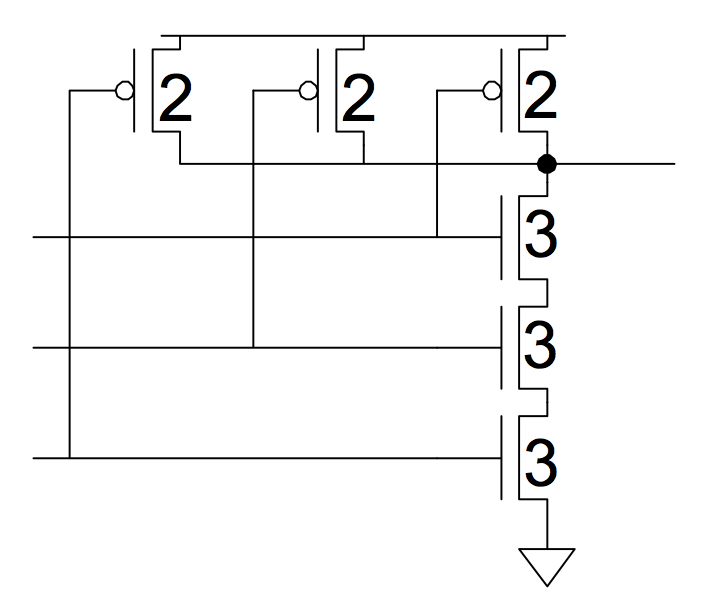
\includegraphics[width=0.7\textwidth]{img/nand_3.jpg}
\caption{Architecture for 3-input NAND gate}
\label{fig:nand_3}
\end{center}
\end{figure}
A 3-input NAND gate with transistor widths chosen to achieve effective rise and fall resistance equal to that of a unit inverter (R). In this case pMOS has a width of $2\cdotp W_N$ (in the worst case, current flows only in one pMOS) to compensate the difference between mobility of electrons and holes, while for nMOS, width is $3\cdotp W_N$ because are in series. \\Now we have to compute the capacitance at each node (neglecting capacitances effect due to layout) shown in figure \ref{fig:nand_3_cap}.
\begin{figure}[htbp]
\begin{center}
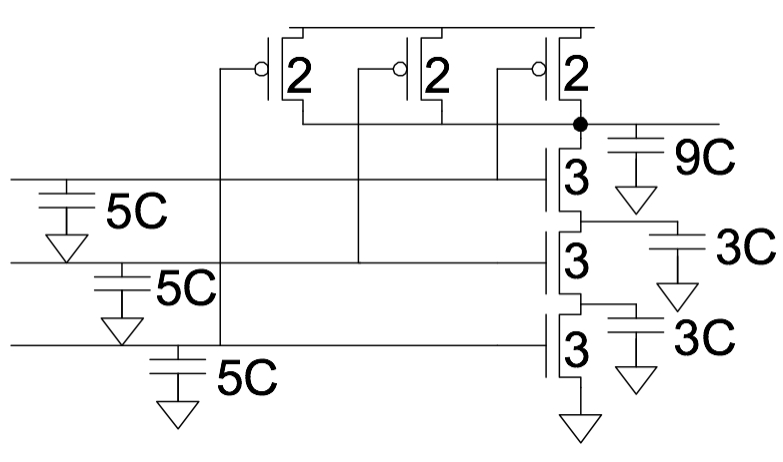
\includegraphics[width=0.7\textwidth]{img/nand_3_cap.jpg}
\caption{Capacitances for 3-input NAND gate}
\label{fig:nand_3_cap}
\end{center}
\end{figure}
As we can see, at each input nodes, capacitances is $5C$ because the aspect ratio is 2 for pMOS and 3 for nMOS, while the output capacitance is $9C$ because the output node is loaded with 3 pMOS and 1 nMOS. Considering layout, the situations is different. In figure \ref{fig:nand_layout}, the source of 2 pMOS are common, so capacitance at output node due to pull-up network is reduced to $4C$, finally the total capacitance is $7C$.
\begin{figure}[htbp]
\begin{center}
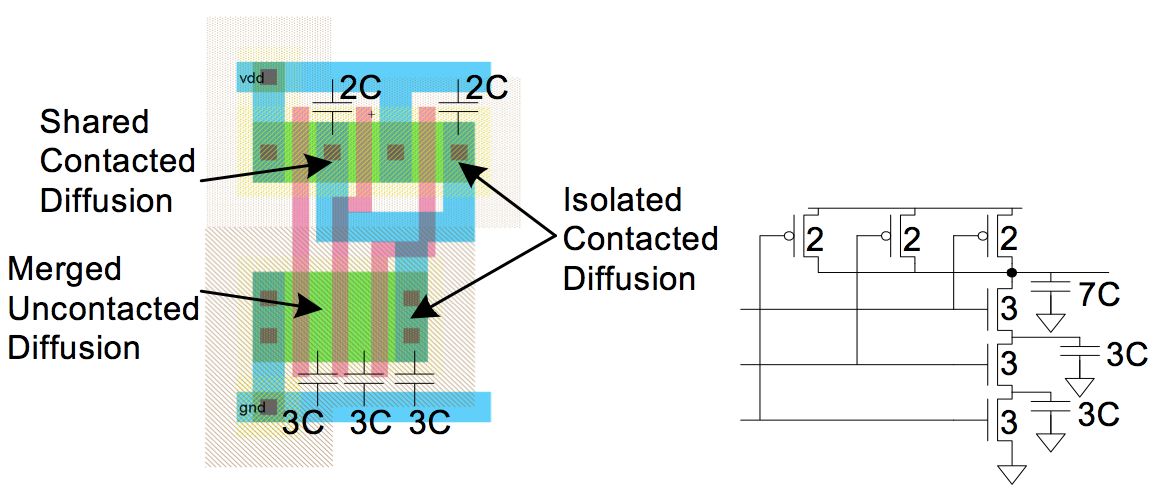
\includegraphics[width=0.9\textwidth]{img/nand_3_layout.jpg}
\caption{Layout example for 3-input NAND gate}
\label{fig:nand_layout}
\end{center}
\end{figure}

For 2-input NAND, we use layout in figure \ref{fig:nand_2_layout}, so the resultant model of capacitances is that in figure \ref{fig:nand_2} where $h$ is the fan-out.
\begin{figure}[htbp]
\begin{center}
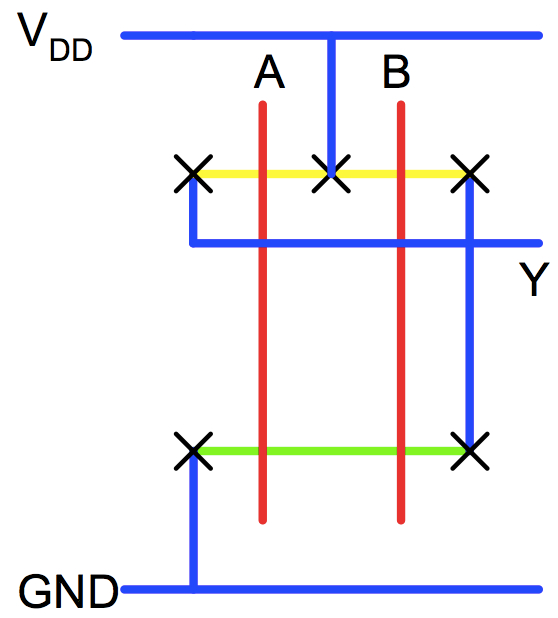
\includegraphics[width=0.4\textwidth]{img/nand_2_layout.jpg}
\caption{Layout for 2-input NAND gate}
\label{fig:nand_2_layout}
\end{center}
\end{figure}
\begin{figure}[htbp]
\begin{center}
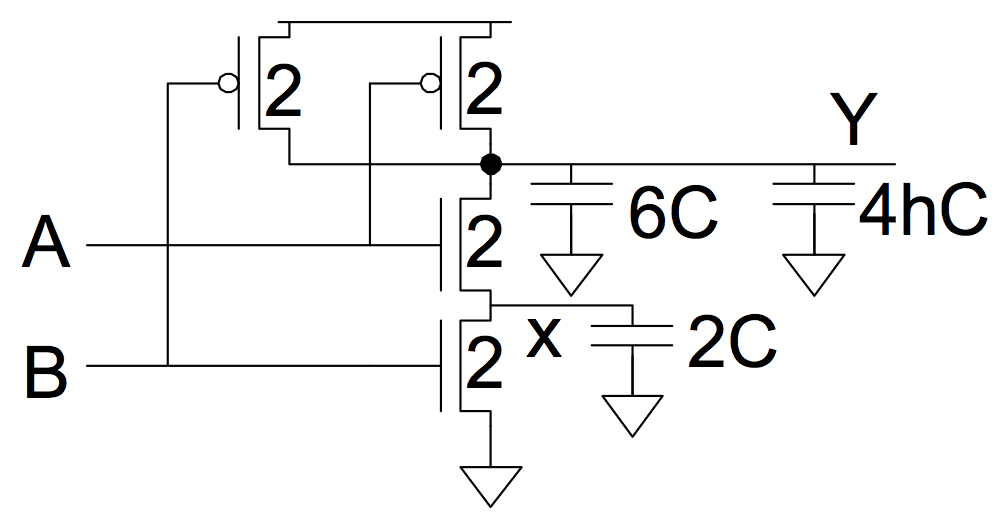
\includegraphics[width=0.7\textwidth]{img/nand_2.jpg}
\caption{Capacitances for 2-input NAND gate}
\label{fig:nand_2}
\end{center}
\end{figure}
Now, let's focus on our formulas to evaluate the delay. First of all it is necessary to estimate equivalent resistance of MOSFET as
\begin{equation}
R=\frac{1}{\mu_n \cdotp C_{OX} \cdotp \frac{W_N}{L_{eff}}\cdotp (V_{DD}-V_{tn})}
\end{equation}
capacitance C is $C_{OUT}$ previously estimated. The rise propagation delay $t_{pdr}$ is
\begin{equation}
t_{pdr}=\biggl(\biggl(2\frac{\mu_p}{\mu_n}+2\biggr)+4\biggr)\cdotp R \cdotp C
\end{equation}
and the fall propagation delay $t_{pdf}$ is
\begin{equation}
t_{pdf}=2\cdotp C \cdotp \frac{R}{2} + \biggl(\biggl(2\frac{\mu_p}{\mu_n}\biggr) + 2 + 4\cdotp h\biggr) \cdotp C \cdotp R
\end{equation}